\documentclass[11pt,compress,t,notes=noshow]{beamer}\usepackage[]{graphicx}\usepackage[]{color}

\makeatletter
\def\maxwidth{ %
  \ifdim\Gin@nat@width>\linewidth
    \linewidth
  \else
    \Gin@nat@width
  \fi
}
\makeatother

\definecolor{fgcolor}{rgb}{0.345, 0.345, 0.345}
\newcommand{\hlnum}[1]{\textcolor[rgb]{0.686,0.059,0.569}{#1}}%
\newcommand{\hlstr}[1]{\textcolor[rgb]{0.192,0.494,0.8}{#1}}%
\newcommand{\hlcom}[1]{\textcolor[rgb]{0.678,0.584,0.686}{\textit{#1}}}%
\newcommand{\hlopt}[1]{\textcolor[rgb]{0,0,0}{#1}}%
\newcommand{\hlstd}[1]{\textcolor[rgb]{0.345,0.345,0.345}{#1}}%
\newcommand{\hlkwa}[1]{\textcolor[rgb]{0.161,0.373,0.58}{\textbf{#1}}}%
\newcommand{\hlkwb}[1]{\textcolor[rgb]{0.69,0.353,0.396}{#1}}%
\newcommand{\hlkwc}[1]{\textcolor[rgb]{0.333,0.667,0.333}{#1}}%
\newcommand{\hlkwd}[1]{\textcolor[rgb]{0.737,0.353,0.396}{\textbf{#1}}}%
\let\hlipl\hlkwb

\usepackage{framed}
\makeatletter
\newenvironment{kframe}{%
 \def\at@end@of@kframe{}%
 \ifinner\ifhmode%
  \def\at@end@of@kframe{\end{minipage}}%
  \begin{minipage}{\columnwidth}%
 \fi\fi%
 \def\FrameCommand##1{\hskip\@totalleftmargin \hskip-\fboxsep
 \colorbox{shadecolor}{##1}\hskip-\fboxsep
     \hskip-\linewidth \hskip-\@totalleftmargin \hskip\columnwidth}%
 \MakeFramed {\advance\hsize-\width
   \@totalleftmargin\z@ \linewidth\hsize
   \@setminipage}}%
 {\par\unskip\endMakeFramed%
 \at@end@of@kframe}
\makeatother

\definecolor{shadecolor}{rgb}{.97, .97, .97}
\definecolor{messagecolor}{rgb}{0, 0, 0}
\definecolor{warningcolor}{rgb}{1, 0, 1}
\definecolor{errorcolor}{rgb}{1, 0, 0}
\definecolor{code}{rgb}{0.97, 0.96, 1.0}
\newenvironment{knitrout}{}{} % an empty environment to be redefined in TeX

\usepackage{alltt}
\usepackage[utf8]{inputenc}
\usepackage[ngerman]{babel}
\usepackage{dsfont}
\usepackage{verbatim}
\usepackage{amsmath}
\usepackage{amsfonts}
\usepackage{mathtools}
\usepackage{csquotes}
\usepackage{cmbright}
\usepackage{multirow}
\usepackage{longtable}
\usepackage{enumerate}
\usepackage[absolute,overlay]{textpos}
\usepackage{psfrag}
\usepackage{algorithm}
\usepackage{algpseudocode}
\usepackage{eqnarray}
\usepackage{bytefield}
\usepackage{animate}
\usepackage{tikz}
\usetikzlibrary{shapes,matrix,positioning,chains,arrows,shadows,decorations.pathmorphing,fit,backgrounds}
\usepackage{adjustbox}
\usepackage{colortbl}
\usepackage{tabularx} % for tables (incl. \hline)
\usepackage{arydshln} % Load after array, longtable, colortab and/or colortbl , otherwise problems with \hline in tabular env
\usepackage{etex} %increase registers for \dimenS to more than 256, otherwise we get "No room for a new \dimen"
\usepackage{graphicx}
\usepackage{booktabs} %used in epr lectures
\usepackage{bm} % bold greek letters
\usepackage{hyperref} % url citing
\usepackage{blkarray} % block arrays
\usepackage{listings} % block of code
\usepackage{xcolor} %colored math symbols
\usepackage{pgffor}
\usepackage{verbatimbox}
\usepackage{xcolor}

%some colors
\definecolor{checkgreen}{HTML}{18A126}
\definecolor{errorred}{HTML}{FF0000}
\definecolor{blockbg}{HTML}{F7F7F7}
\definecolor{gray}{HTML}{A0A0A0}

% basic latex stuff
\newcommand{\col}{\par\colorbox{code}{\parbox{\textwidth}{\theverbbox}}\par}
\newcommand{\eg}{e.\,g.\xspace} %for example
\newcommand{\ie}{i.\,e.\xspace} %that is to say...
\newcommand{\pkg}[1]{{\fontseries{b}\selectfont #1}} %fontstyle for R packages
\newcommand{\lz}{\vspace{0.5cm}} %vertical space
\newcommand{\oneliner}[1] % Oneliner for important statements
{\begin{block}{}\begin{center}\begin{Large}#1\end{Large}\end{center}\end{block}}
\def\SpAr{\quad \Rightarrow \quad}

%new environments
\newenvironment{vbframe}  %frame with breaks and verbatim
{
 \begin{frame}[containsverbatim,allowframebreaks]
}
{
\end{frame}
}

\newenvironment{vframe}  %frame with verbatim without breaks (to avoid numbering one slided frames)
{
 \begin{frame}[containsverbatim]
}
{
\end{frame}
}

\newenvironment{blocki}[1]   % itemize block
{
 \begin{block}{#1}\begin{itemize}
}
{
\end{itemize}\end{block}
}

\newenvironment{fragileframe}[2]{  %fragile frame with framebreaks
\begin{frame}[allowframebreaks, fragile, environment = fragileframe]
\frametitle{#1}
#2}
{\end{frame}}

\newcommand{\myframe}[2]{  %short for frame with framebreaks
\begin{frame}[allowframebreaks]
\frametitle{#1}
#2
\end{frame}}

\usepackage{../../style/lmu-lecture}

\let\code=\texttt
\let\proglang=\textsf

\setkeys{Gin}{width=0.9\textwidth}

\usepackage{tikz}
\usetikzlibrary{shapes,arrows,snakes, calc}

% Define block styles
\tikzstyle{decision} = [diamond, draw, text width=6em, text badly centered, node distance=4cm, inner sep=0pt]
\tikzstyle{decision2} = [diamond, draw, fill=customgreen!35, text width=6em, text badly centered, node distance=4cm, inner sep=0pt]

\tikzstyle{block} = [rectangle, draw, text width=14em, text centered, rounded corners, node distance=3cm, minimum height=4em]
\tikzstyle{line} = [draw, -latex']
\tikzstyle{cloud} = [draw, ellipse, node distance=3cm, minimum height=2em]

\title{Introduction to Deep Learning}
\author{Bernd Bischl}
\institute{Department of Statistics -- LMU Munich}
\date{WS 2021/2022}

\setbeamertemplate{frametitle}{\expandafter\uppercase\expandafter\insertframetitle}

\IfFileExists{upquote.sty}{\usepackage{upquote}}{}
\input{../../latex-math/basic-math}
\input{../../latex-math/basic-ml}
\input{../../latex-math/ml-nn}

\title{Deep Learning}

\date{}

\begin{document}
\newcommand{\titlefigure}{plots/FigureDice}
%modify picture
\newcommand{\learninggoals}{
  \item probabilistic graphical models
  \item latent variables
  \item directed graphical models 
  %\item adversarial training 
  %\item projected gradient descent
  %\item fast gradient sign method
  %\item Principal component analysis
}

\lecturechapter{Probabilistic graphical models}
\lecture{I2DL}



\section{Probabilistic graphical models}



\begin{frame}{Graphical models}
    
    
    \begin{center}
    \begin{minipage}{.9\textwidth}
    \begin{block}{}
    \begin{center}
    \textbf{Probabilistic graphical models}
    describe probability distributions
    by mapping conditional dependence and independence properties
    between random variables
    on a graph structure.
    \end{center}
    \end{block}
    \end{minipage}
    \end{center}

\end{frame}



\begin{frame}{Why again graphical models?}
    
    \begin{minipage}{.62\textwidth}
    \begin{enumerate}\itemsep2ex
    \item Graphical models visualize the structure of a probabilistic
    model; they help to develop, understand and motivate probabilistic models.
    %\item Die Graphstruktur macht wichtige Eigenschaften der Verteilung
    % deutlich, insbesondere bedingte Abhängigkeiten und Unabhängigkeiten.
    \pause
    \item Complex computations (e.g., marginalization)
    can derived efficiently
    using algorithms exploiting the graph structure.
    \end{enumerate}
    \end{minipage}
    \hfill\begin{minipage}{.33\textwidth}
    \phantom{mini}
    
    \hfill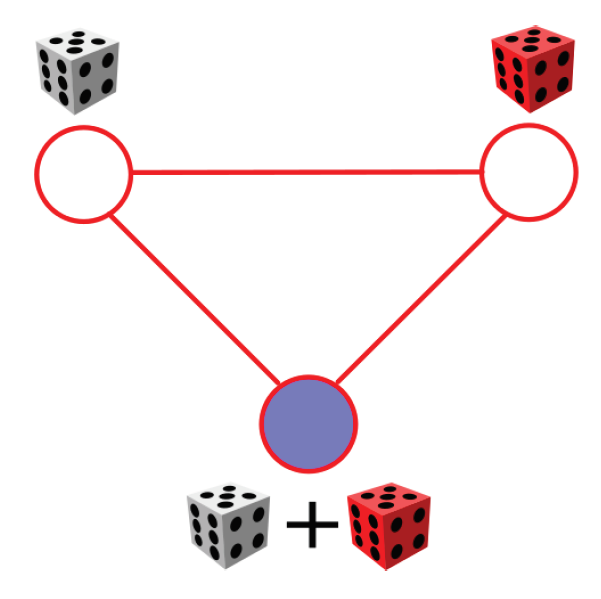
\includegraphics[width=.95\textwidth]{plots/FigureDice}
    \end{minipage}

\end{frame}

\begin{frame}{Graphical models: Example}

  \begin{figure}
    \centering
    \scalebox{0.9}{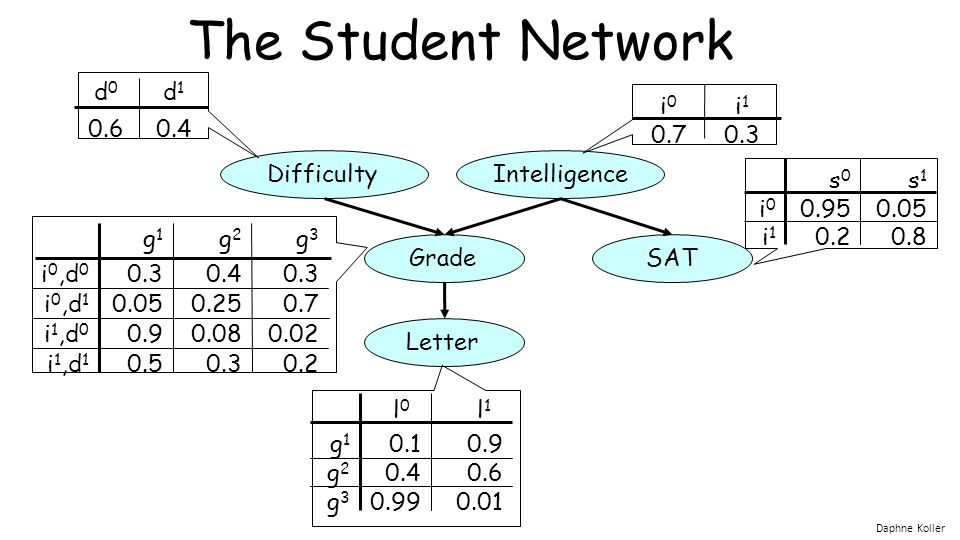
\includegraphics{plots/studnet.png}}
    \tiny{\\Credit: Daphne Koller}
    \caption{\footnotesize A graphical model representing five variables and their (in-)dependencies along with the corresponding marginal and conditional distributions. The variable 'Grade', for example, is affected by 'Difficulty' (of the exam) and 'Intelligence' (of the student). This is captured in the corresponding conditional distribution. 'Letter' refers to a letter of recommendation. In this model, 'Letter' is conditionally independent of 'Difficulty' and 'Intelligence', given 'Grade'.}
  \end{figure}

\end{frame}


\section{Latent Variables}

% \frame{
%     \frametitle{Latent variables: Motivation}
%     
%     \mode<beamer>{\begin{center}
%         \only<1>{
\includegraphics[width=7cm]{plots/ImCrossO.pdf}}\only<2>{
\includegraphics[width=7cm]{plots/ImHeartR.pdf}}\only<3>{
\includegraphics[width=7cm]{plots/ImStarO.pdf}}\only<4>{
\includegraphics[width=7cm]{plots/ImCrossR.pdf}}\only<5>{
\includegraphics[width=7cm]{plots/ImStarB.pdf}}\only<6>{
\includegraphics[width=7cm]{plots/ImStarR.pdf}}
%         \end{center}}
%     \mode<handout>{\begin{center}
%         
\includegraphics[width=7cm]{plots/ImCrossO.pdf}
%         \end{center}}
%     
%     \begin{center}
%     $200\times 200$ pixels \quad$\rightarrow$\quad
%     $2^{40000}-1$ parameters?
%         \end{center}
% }

\begin{frame}{Latent variables: Motivation}
  \begin{figure}
    \centering
      \scalebox{0.8}{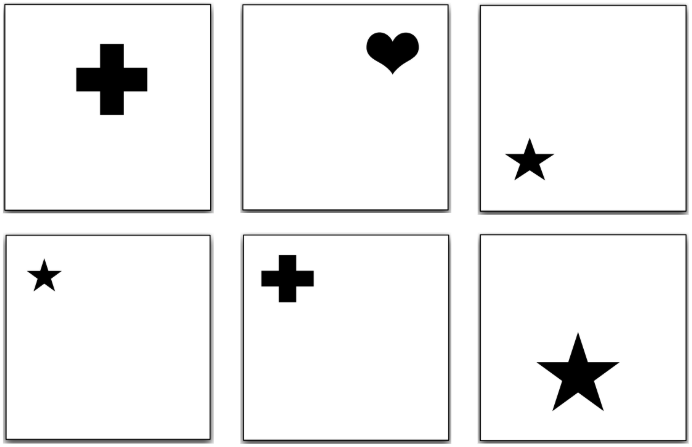
\includegraphics{plots/latvar_motiv.png}}
\caption{\footnotesize A simple illustration of the relevance of latent variables. Here, six 200 x 200 pixel images are shown where each pixel is either black or white. Naively, the probability distribution over the space of all such images would need $2^{40000}-1$ parameters to fully specify. However, we see that the images have three main factors of variation : object type (shape), position and size. This suggests that the actual number of parameters required might be significantly fewer. }
 \end{figure}
\end{frame}


 
\frame{
    \frametitle{Latent variables}
    \begin{itemize}
    \item Additional nodes, which do not directly correspond
    to observations, allow to describe complex distributions
    over the visible variables by means of simple conditional distributions.
    \item The corresponding random variables are called \emph{hidden} or
    \emph{latent} variables.
    \end{itemize}
    
    \begin{center}
    \begin{figure}
    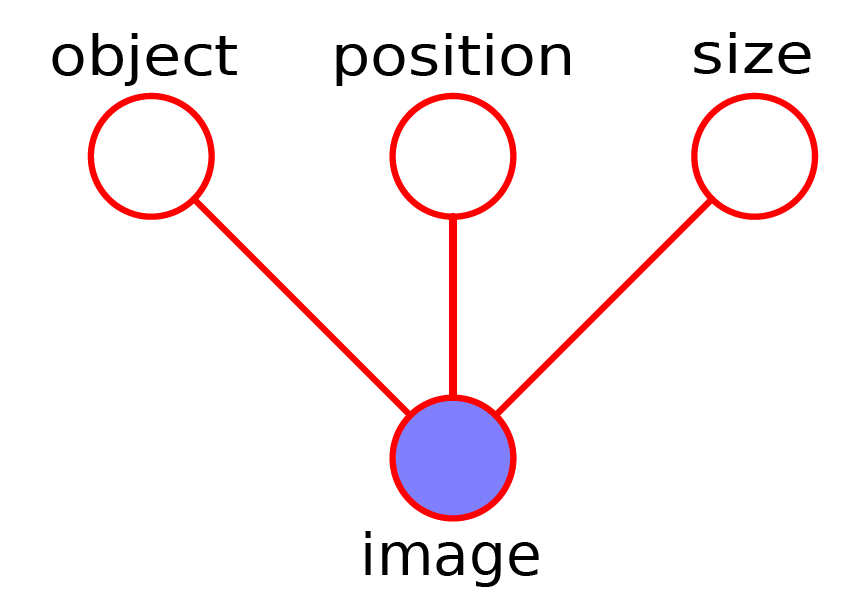
\includegraphics[width=5cm]{plots/MyFigure8-8}
    \caption{\footnotesize 'Object', 'position' and 'size' are the latent variables behind an image.}
    \end{figure}
    \end{center}
    
}



\section{Directed generative models}


\frame{
    \frametitle{Directed generative models}
    
    \textbf{Goal:} Learn to generate $\xv$ from some latent variables $\mathbf{z}$
    
    $$p_{\thetab}(\xv) = \int p_{\thetab}(\xv, \mathbf{z}) d\mathbf{z} = \int p_{\thetab}(\xv| \mathbf{z}) p_{\thetab}(\mathbf{z}) d\mathbf{z}$$
        
        %Todo: h zu z machen, theta einbauen moeglich?!!!
        \begin{figure}
    %\hspace{-3cm}
    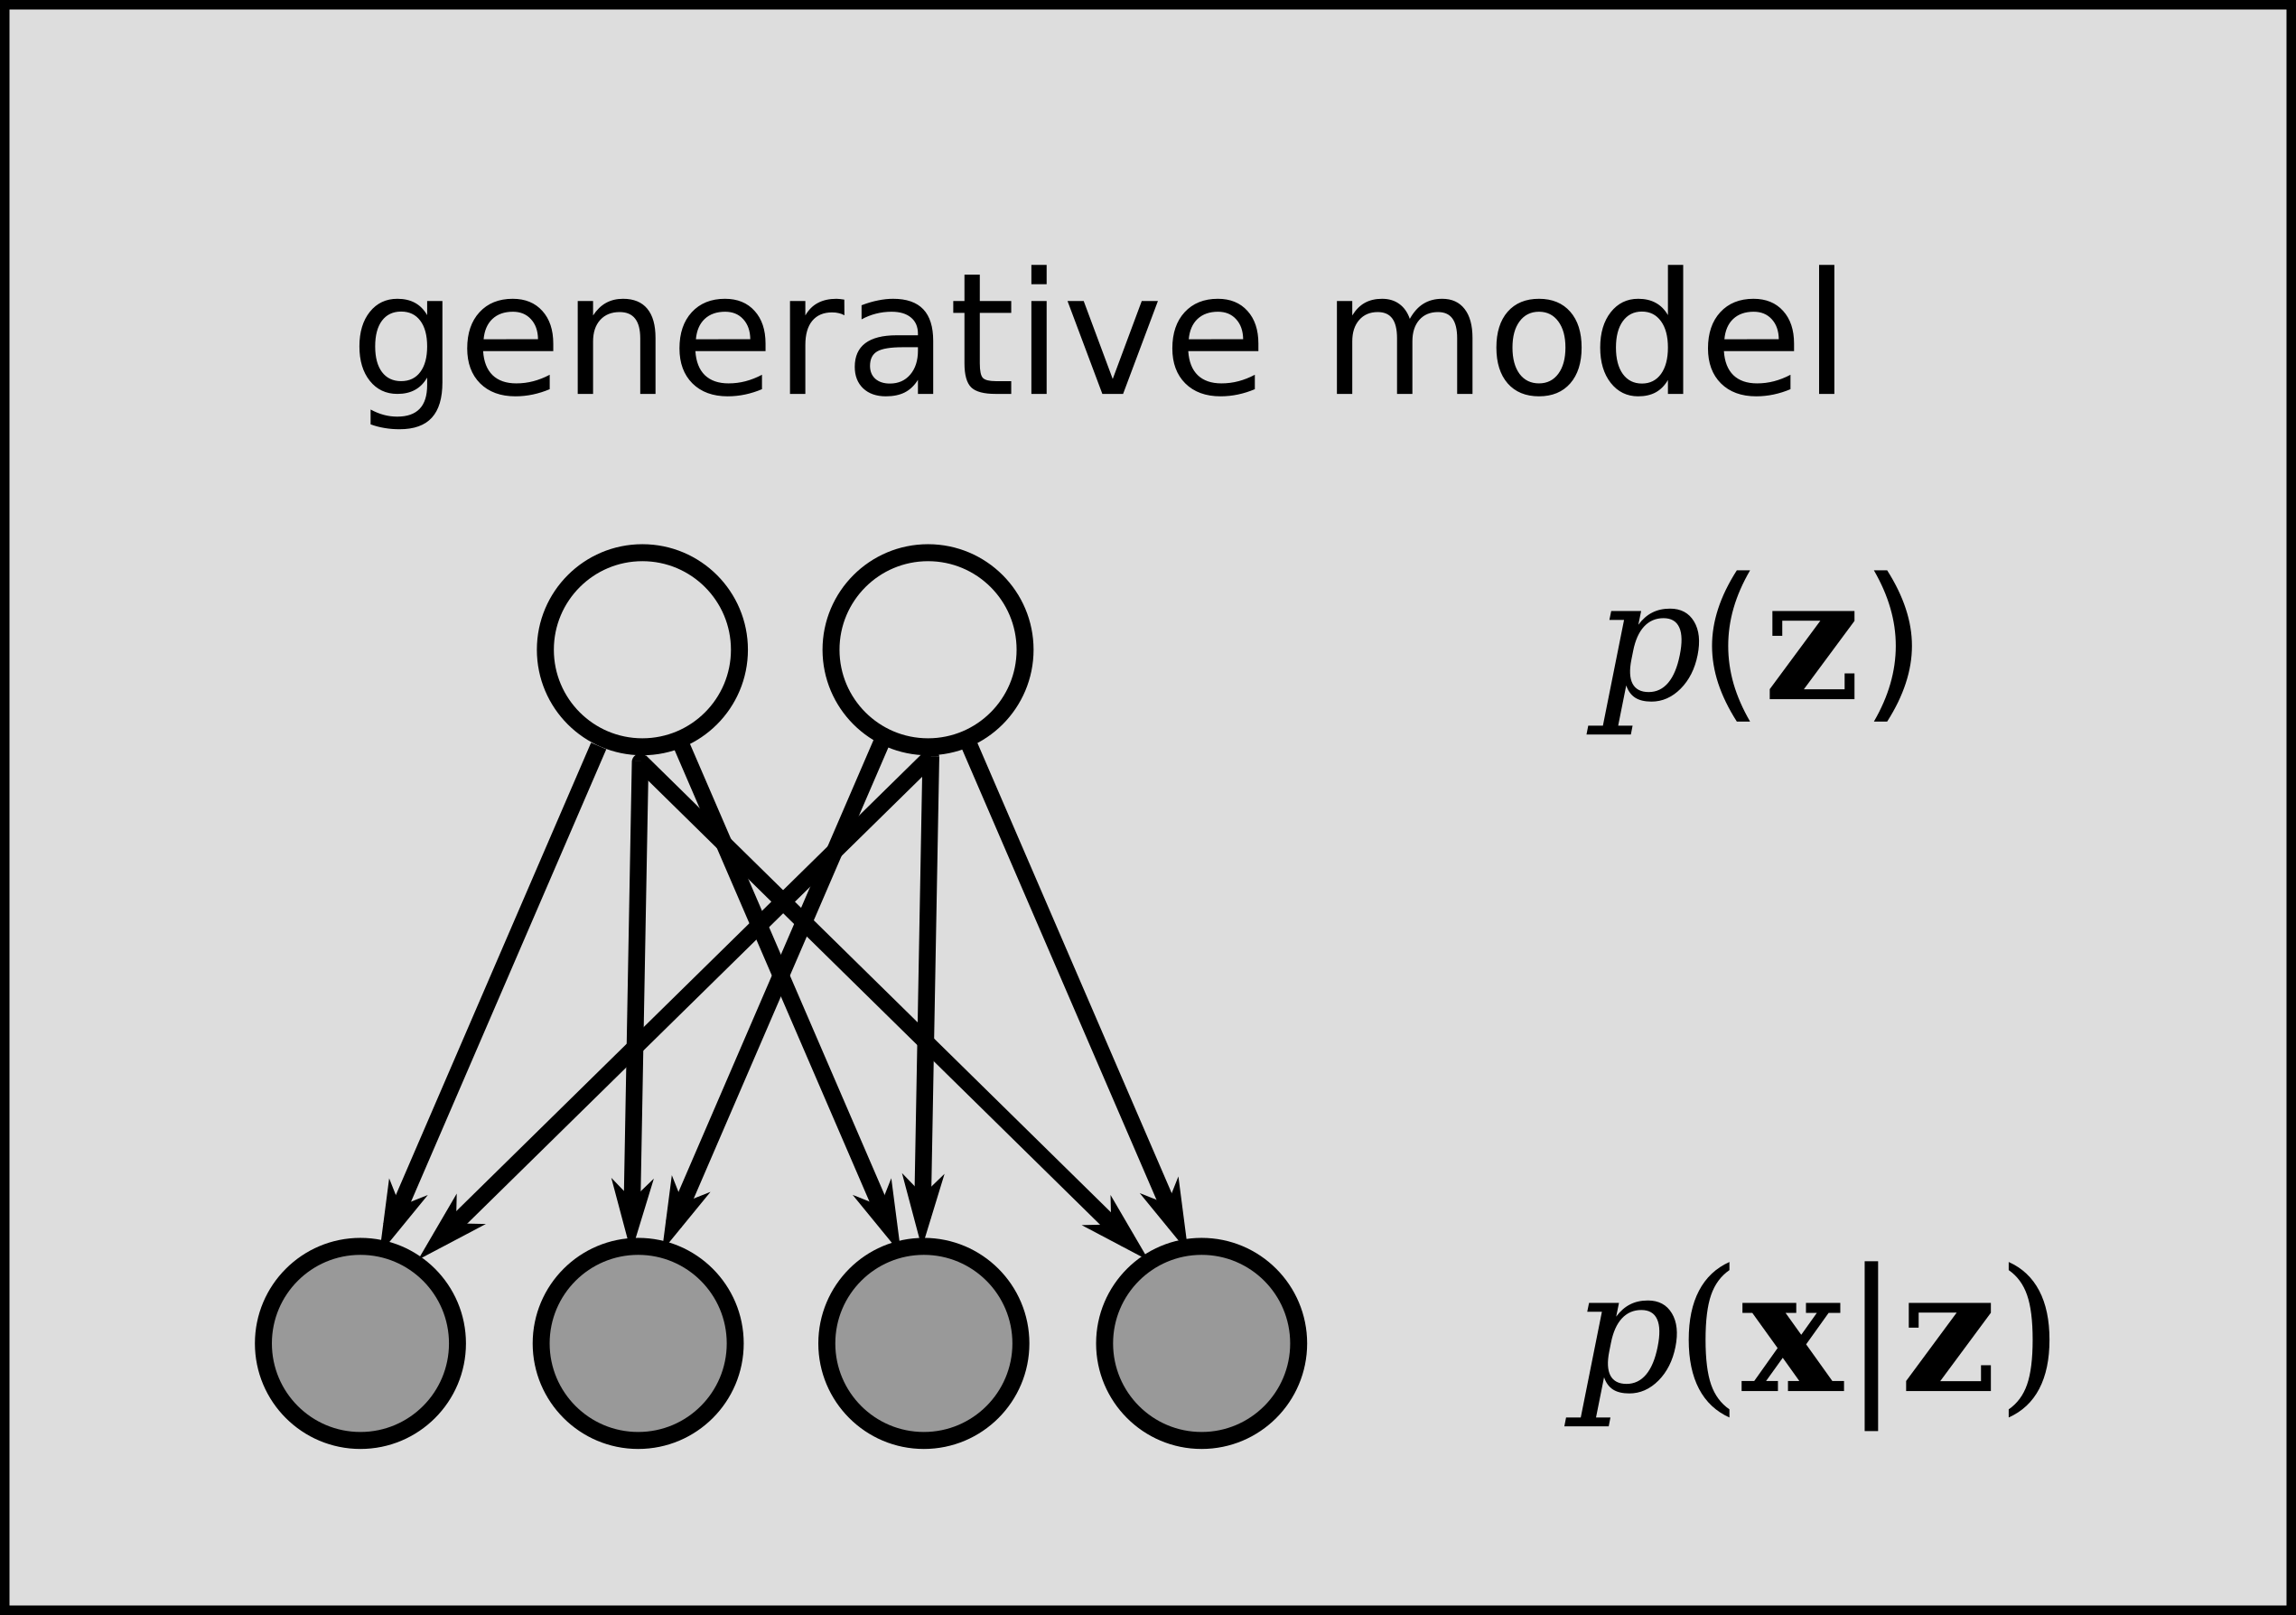
\includegraphics[width=4cm]{plots/VAE.png}
    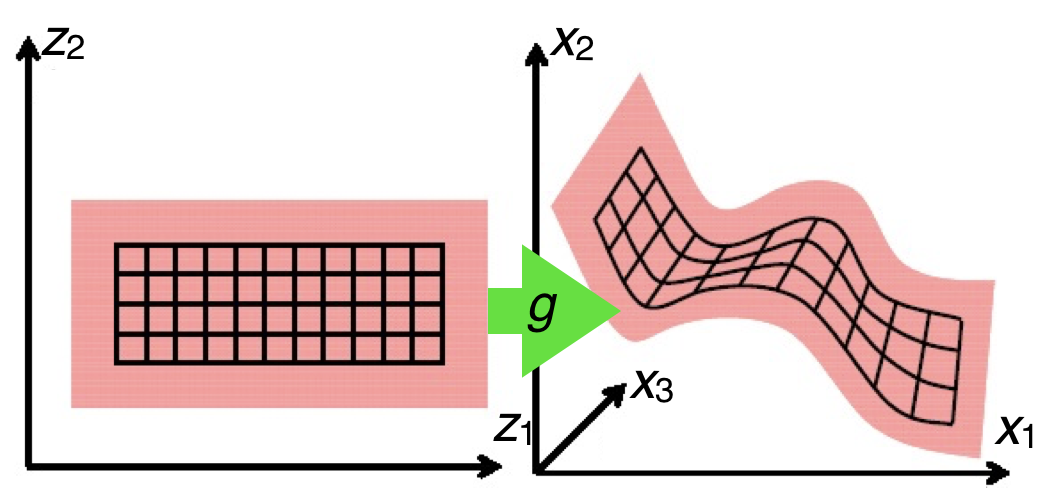
\includegraphics[width=7cm]{plots/zToxManifold.png}
    \tiny{Image from: Ward, A. D., Hamarneh, G.: \textbf{3D Surface Parameterization Using Manifold Learning for Medial Shape Representation}, Conference on Image Processing, Proc. of SPIE Medical Imaging, 2007}
    \caption{\footnotesize \textit{Left}: An illustration of a directed generative model. \textit{Right}: A mapping (represented by $g$) from the 2D latent space to the 3D space of observed variables.}
    \end{figure}
    
    
    
}

\frame{
    \frametitle{Directed generative models}
    
     The latent variables $\mathbf{z}$ must be learned from the data (which only contains the observed variables $\xv$).
        
        \begin{itemize}
    \item %For inference we need
    The posterior  is given by $p_{\thetab}(\mathbf{z}| \xv ) = \frac{p_{\thetab}(\xv| \mathbf{z})p_{\thetab}(\mathbf{z})}{p_{\thetab}(\xv)}$.
    %
    % \pause
    \item But $p_{\thetab}(\xv)=\int p_{\thetab}(\xv|\mathbf{z}) p_{\thetab}(\mathbf{z}) d\mathbf{z}$ is intractable and common algorithms (such as Expectation Maximization) cannot be used.
    \end{itemize}
    
    \pause
    
    The classic DAG problem: How do we efficiently learn $p_{\thetab}(\mathbf{z}| \xv )$?
    %An VAE contains two directed graphical models
    %An VAE  consists of directed graphical models
    
    %\vspace{0.7cm}
    %\only<1-3>{\hspace{2,3cm
        \hspace{3.3cm}
        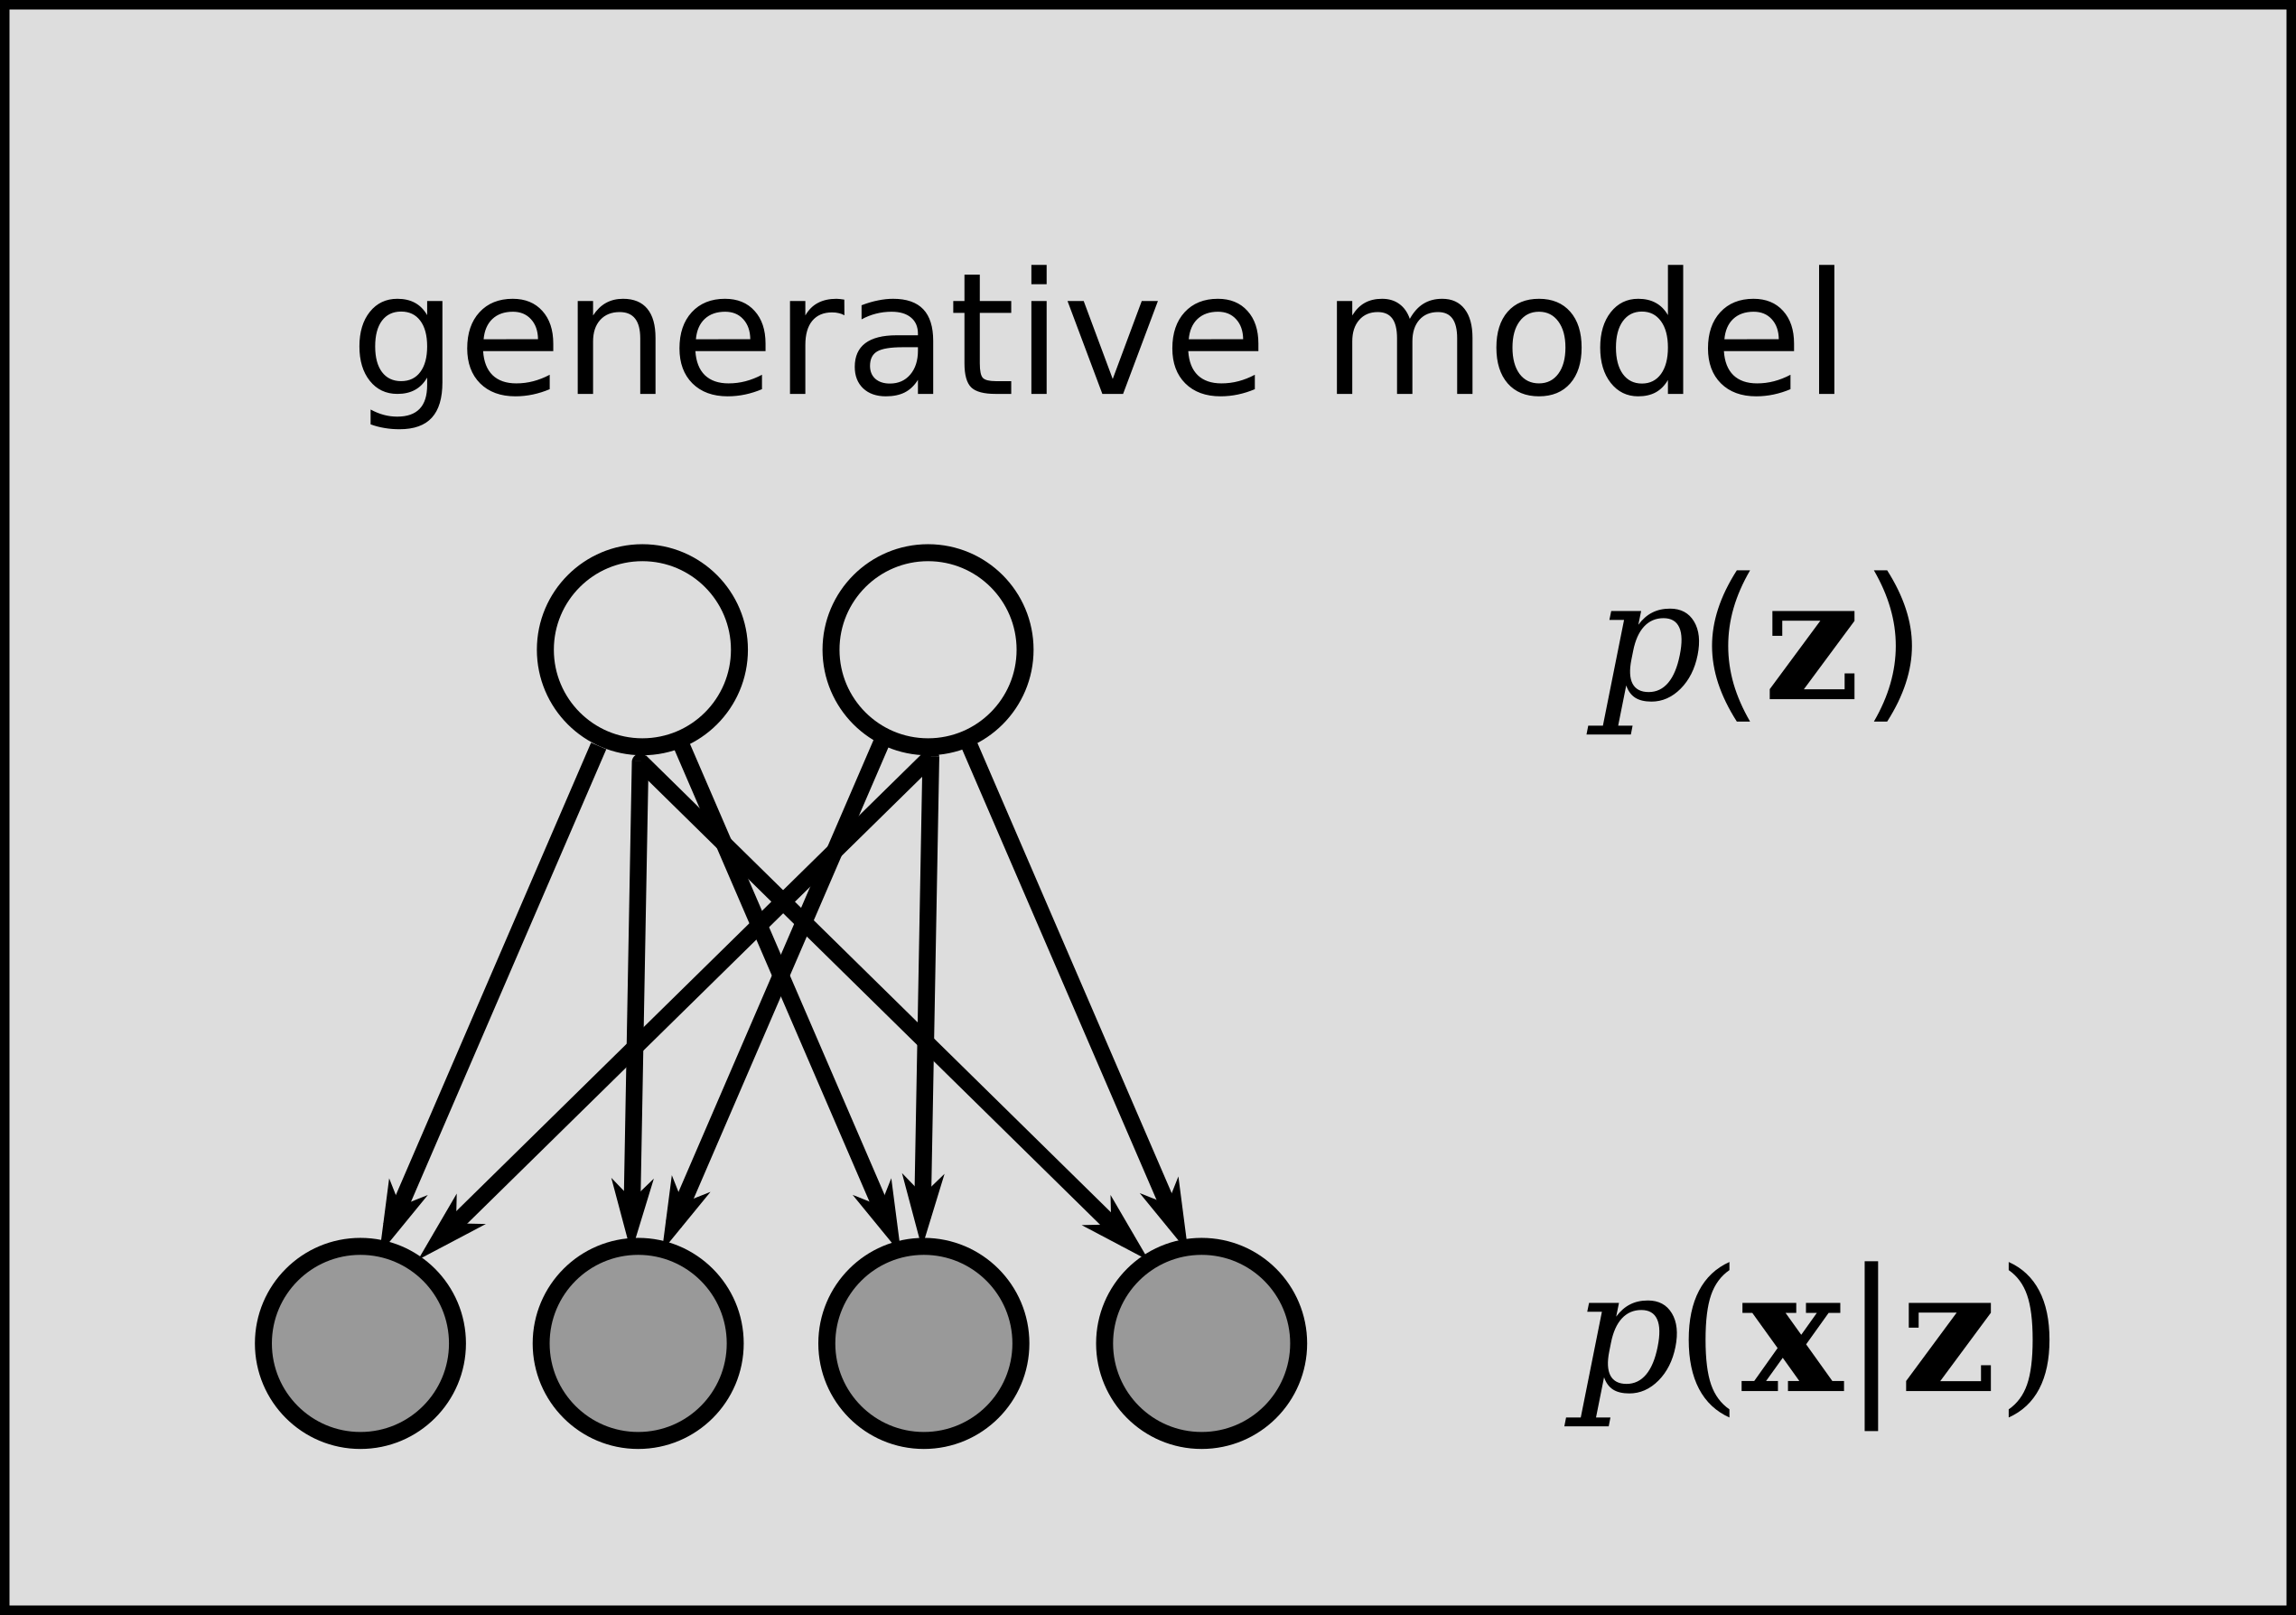
\includegraphics[width=0.37\framewidth]{plots/VAE.png}
        
        Popular approaches to this problem:
            \begin{itemize}
        \item \textbf{Variational Autoencoders (VAEs)}
        \item \textbf{Generative Adversarial Networks (GANs)}
        \end{itemize}
        
    }
%%%%%%%%%%%%%%%%%%%%%%%%%%%%%%%%%%%%%%%%%%%%%%%%%%%%%%%%%%%%%%%%%%
%%%%%%%%%%%%%%%%%%          REFERENCES          %%%%%%%%%%%%%%%%%%
%%%%%%%%%%%%%%%%%%%%%%%%%%%%%%%%%%%%%%%%%%%%%%%%%%%%%%%%%%%%%%%%%%



%%%%%%%%%%%%%%%%%%%%%%%%%%%%%%%%%%%%%%%%%%%%%%%%%%%%%%%%%%%%%%%%%%
%%%%%%%%%%%%%%%%%%%%%%%%%%%%%%%%%%%%%%%%%%%%%%%%%%%%%%%%%%%%%%%%%%

\endlecture
\end{document}